\documentclass[11pt]{article}
\usepackage[margin=1in]{geometry}          
\usepackage{graphicx}
\usepackage{amsthm, amsmath, amssymb}
\usepackage[font=small]{caption, subcaption}
\usepackage{setspace}\onehalfspacing
\usepackage[loose,nice]{units}
\usepackage{array}
\usepackage[super]{nth}
\usepackage{graphicx}
\usepackage{float}
\usepackage{cleveref}
\usepackage{subcaption}
\usepackage{mathtools}
\usepackage[displaymath, mathlines]{lineno}
\usepackage{natbib}
\usepackage[all]{nowidow}
\usepackage{wrapfig}
\usepackage{pdfpages}
\newenvironment{conditions}
  {\par\vspace{\abovedisplayskip}\noindent\begin{tabular}{>{$}l<{$} @{${}={}$} l}}
  {\end{tabular}\par\vspace{\belowdisplayskip}}
\newcommand{\R}{\mathbb{R}}  
\DeclareMathOperator*{\E}{\mathbb{E}}
 
\author{
	Dr. Yoav Ram
	\and
	Saar Egozi
}
 
\begin{document}

\begin{titlepage}
\centering

\vspace{4cm}

{\LARGE\bfseries Prestige as a Driving Force in Cultural Transmission}

\vspace{2cm}

{\large\bfseries Saar Egozi}

\vspace{1cm}

{\large together with Yoav Ram}

\vspace{2cm}

\vfill

{\large Efi Arazi School of Computer Science, IDC Herzliya}

\vspace{1cm}

{\itshape \today}

{\large saartk@gmail.com}
\end{titlepage}


\renewcommand\linenumberfont{\normalfont\small\sffamily}
\linenumbers
\modulolinenumbers[2]
\setcounter{secnumdepth}{0}
\tableofcontents

\clearpage

\section{Abstract}
Copying our role-models have always been an efficient method of acquiring knowledge. Copying successful role-model is one of the methods of cultural transmission of traits. In this paper, we study the various biases and their effects of the population and it's evolution. The most common bias when choosing a role-model to copy is \textit{success bias}, i.e copying whoever appears successful to us. This estimation is based on the performance of the role-model alone, without any other factors. Here, we study another factor we believe aids to better model the cultural inheritance of traits in a large population. \textit{Influence bias} is a bias evaluated by the number of copiers a role-model already has. In our model we combine these components to what we call the \textbf{Prestige bias} and analyze its relationship to the dynamics of the population. We successfully found mathematical approximations to our model, easing the mathematical analysis and the computation power required for simulations. We show the value of these approximations using simulations, and their robustness to variations such as mutation and other relaxations required for the mathematical proofs.
In the binary form of our model, we found alternatives to \textit{Kimura's} equations for approximating fixation probability and time to fixation of an invading advantageous trait, in both a constant and changing environment. We show that \textit{Influence} solely affects the effective population size.
We found that influence acts as an accelerator for a state of the population, matching the \textit{rich getting richer} it was based on.
We believe such model better describes how humans acquire knowledge from one another, mainly in the last years where social networks are very popular. Social networks allow easy access to estimate number of copiers a role-model has, with little to no effort.

% what is cultural transmission, and its not only in humans
\section{Introduction}
Traits transmission is when an individual passes on a trait, genetic or behavioral, to another individual. Transmission in nature manifests in two main ways: genetic and cultural.
Genetic transmission is when an individual, or several, transmit their genes to their offspring by duplication of their own cells.
Cultural transmission is the way individuals transmit cultural traits (i.e behavior) from one another, typically via teaching and demonstrating.
 Cultural transmission is most common in humans \citep[pg. 3]{transmissionVectorsBook} and in primates like chimpanzees \citep{chimpsPrestige, chimpsCopy}.
 The common cultural traits in humans are behavioral patterns, like personalities and habits, transmitted via observations and verbal discussions.
\citet{dualEvolution} suggest that cultural learning may be particular to humans, but \citet{elepahntsRepo} suggest that it appears in other mammals as well, elephants for example:
 \begin{quote}
	   ... the possession of enhanced discriminatory abilities by the oldest individual [matriarch] in a group can influence the social knowledge of the group as a whole.
 \end{quote}
 They showed that once a matriarch is removed from the group, the group's survival instincts are inferior.
 They support their hypothesis by exacting an experiment: playing audio recordings of African elephants, showing that groups with a matriarch recognize and react better to hostile or friendly calls than the groups without one.
Moreover, cultural transmission appears in other species, even simpler than mammals, such as \textit{Drosophila}.
\citet{fliesPaper} show that oviposition site choice in fruit flies is culturally transmitted.
They showed that flies without experience in choosing sites, after spending some time with "experienced" flies, chose the same type of site without directly observing this behavior. 
\citet{fliesPaper} mention that how the information is transferred is still an open question, but suggest that the flies may use olfactory cues, like other animals such as rodents and bees.\\ 

%the differences and similarities between cultural and genetic transmission 
Cultural transmission is similar to genetic transmission in many ways, while different in others.
Similar to genetic transmission, the effects of culturally transmitted traits can be physiological rather than behavioral, and transmitted from parents to offspring.
 For example, parents can teach their children to be strong or tall, within some biological limits, by instructing them to maintain a healthy diet and engage in physical activity.
Contrary to genetic transmission, the sources of the traits can be many, and not only parents. They can even be unrelated, like teachers, celebrities, coaches, the media, or any stranger that comes in contact with them. 
 Cultural transmission can be vertical, where parents transmit to their children, but also oblique, where other adults transmit traits to children (not their own).
  Horizontal transmission is also possible, where peers transmit traits to one another. 
   Lastly, vertical transmission in the opposite direction is possible too, where parents copy traits from their children (e.g playing video games) as \citet{transmissionVectorsBook} and \citet{transmissionVectors} suggest. 
In addition, even when a cultural trait is disfavored by natural selection, it still may spread across a population given transmission biases strong enough to negate the selection bias \citep[Ch. 8 pg. 279]{evolutionBook}.\\ 

%transmission biases - what they are, what are the types.
Transmission bias occurs when a trait has a disproportionate probability from its frequency in the population to be transmitted.
For example, \citet{wtfGene} show that there are genes of yeast called \textit{wtf genes}, that bias their transmission to the gametes.
They secrete a long life expectancy poison, together with a short life expectancy antidote, so a gamete without the gene will perish (the poison will outlive the antidote).
Transmission biases, though exist in genetic transmission, are probably more common in cultural transmission.
Much like mutation in genetic evolution, one could learn behavioral patterns or traits on his own, usually referred to as \textit{innovation}, also called individual learning, and just like mutation, without it humans might have been remained at the stone age, or even go extinct.
\citet{strategiesPaper} suggest that success biased social transmission contribute more to the general success of the population than individual learning.
 They conducted a tournament for developing learning strategies of a population, where each participant need to devise a strategy.
 Each strategy must define when individuals should observe and copy from others, and when to engage in individual learning.
 The best strategies contained a high percentage of social learning relative to individual learning, even when the error when copying was as high as almost 0.5. It is important to add that all of the strategies include some percentage of individual learning, and without it the results would be a lot worse.
In addition to \citet{strategiesPaper}, \citet{complexityPaper} define different types of transmission biases based on success.
They define several types of role-model choosing methods, all assuming that the copier correctly identifies the successful ones.
Both studies assume that individuals can successfully evaluate successful individuals.
\citet[Ch. 5]{evolutionBook} suggest that the \textbf{evaluation} of success can be divided into three groups: \textit{direct bias}, \textit{indirect bias} and \textit{frequency-dependent bias}.
A direct bias is when a variation of a trait is more attractive than others, and is evaluated by \textit{directly} testing the variation of the trait.
For example, an individual observing a Ping-Pong match between two others can try both of the paddle grips it observed, and decide what grip is better for it.
An indirect bias is when an individual uses the value of one trait to determine the attractiveness of another, so it \textit{indirectly} evaluates the attractiveness of the role-model.
Continuing with the example, a bystander could copy the paddle grip of the Ping-Pong player who scored more points in the match.
A frequency-dependent bias is when an individual has a probability to copy a variant of the trait that is nonlinear to the trait's frequency in the parent's generation. 
Continuing with the example, when an individual is 80\% likely to copy the common paddle grip even when only 60\% of the population is using it, it is said to be frequency-biased.\\
Frequency bias could be negative too. \citet{negativeFrequency} show that societies under competitive conditions are likely to develop diversity in foraging specialization rather than uniformity.
 
%prestige bias - what is it, what's missing
Prestige means having a good reputation or high-esteem, therefore does not directly signify success (although it may imply it), making it an \textit{indirect bias}.
Both \citet[Ch. 8]{evolutionBook} and \citet{complexityPaper} claim that prestige biases are probably more common in humans than success biases.
\citet[Ch. 8]{evolutionBook} add that maladaptive traits may spread widely in a population, if the indirect bias is strong enough.
They claim the bias could lead to a \textit{runaway process}, caused by a cultural equivalent of \textit{sexual selection} \citep{sexualSelectionBook}.
On the other hand, \citet{henrichBroesch} claim that prestige biases, over generations, can lead to cultural adaptations.
According to them, prestige can make a maladaptive trait spread in the population, but can also accelerate the spread of adaptive traits as well.
\textit{Prestige bias} is often mentioned in the literature, but seldom modeled.
\citet{evolutionBook} have modeled the prestige bias, but didn't include the effects the copiers of a role-model has on the probability of other individuals to choose the same role model.\\
This effect is similar to \textit{conformity} \citep{conformity}, which is usually modeled as a different bias.
\textit{Conformist learning} (imitating locally common behaviors) is a known bias in cultural transmission \citep{conformism}, and we suggest that prestige bias is made up by both indirect bias and a new type of conformity.
Our new component, \textit{influence}, is assigned to a role-model, contrary to conformity, which refers to the frequency of a trait in the population, regardless which individuals posses it.
\textbf{The goal of this study is to define a more realistic model for prestige bias and analyze the dynamics of the population it causes}.
 
Today, due to social media, it is easier than ever to estimate the influence individuals have over others, therefore it is probably a major part of humans decision-making process. For example, the number of \textit{followers} a person has in the mobile application \textit{Instagram} may significantly affect how his beliefs are perceived by the population.
We want to create a model that better fits reality and simulate scenarios that better mimic cultural transmission dynamics.
With a more accurate model of prestige bias, we may understand better how cultural traits are transmitted, and why.
Moreover, we could better explain the cause for the spread of maladaptive traits, or the acceleration of adaptive traits often seen in humans.


\section{Models and Methods}
\paragraph{Reminder:} A \textit{Wright–Fisher model} is a mathematical model meant to describe a genetic drift process. This model assumes that generations do not overlap and that each copy of the gene found in the new generation is drawn independently at random from all copies of the gene in the old generation.

A \textit{Moran model} assumes overlapping generations. At each time step, one individual is chosen to reproduce and one individual is chosen to die. In our models we harness these two models and modify them to describe new mathematical models that we use to expand the basic indirect bias model \citet{evolutionBook} suggest.

\subsection{Continuous Model}
Consider a population of N individuals, each individual has one trait on a continuous scale. Every generation, $N$ naive individuals (\textit{copiers}) must choose a trait to copy from one of the individuals of the previous generation (\textit{role-models}). Similar to a Wright–Fisher model, we assume the generations don’t overlap. We base our model on the model of \citet{evolutionBook}, by assuming only oblique transmission of the traits (\textit{Indicator trait - A}). Unlike their model, we omit a second trait called \textbf{Indirectly biased trait} to lower complexity. The model’s state at time $t$ can be described by:
\begin{equation}
\vec{A}_t=(A_{t,1}, \ldots, A_{t,N})
\end{equation}
where $\vec{A}_t$ is a vector describing the indicator traits at time $t$, and $\vec{A}_0$ is drawn from a standard normal distribution.
Each individual from generation $t+1$, a \textit{copier}, inherits traits like so:
\begin{equation}
A_i' = F_i(\vec{A}_t)
\end{equation}
where $A_i'$ is the indicator and indirect trait values correspondingly, that copier $i$ acquires.
We use $A_i'$ as an alias for $A_{i,(t+1)}$ for simplicity for the transition between generations $t \rightarrow t+1$.
$F$ is a function over the $t$ generation traits vector, and is defined differently for every implementation of the \textbf{Generic model}.

\paragraph{Success bias.} \citet[Ch.8, p.247-249]{evolutionBook} describe a method of inheritance using a \textit{blend}, i.e weighted average of the trait of the entire generation. They define $F$ as a weighted average  of the role-models' traits in a single generation:
\begin{equation}
F_i(\vec{X}) = \sum_{j=1}^N \Big(G_{ij}\cdot X_{ij}\Big) \\
\end{equation}
where $G_{i,j}$ is: 
\begin{equation}
G_{ij} = \frac{\beta(A_{ij})}{\sum_{l=1}^{N} \beta(A_{il})}
\end{equation}
We define $G_{ij}$ to be the \textit{Success bias} of role-model $j$ in the eyes of copier $i$.
$A_{i,j}$ is the absolute indicator trait value copier $i$ estimates role-model $j$ has:
\begin{equation}\label{eq:relativeIndicator}
A_{i,j} = A_j + e_i,
\end{equation}
where $e_i$ is the copier's error of estimation, $\vec{e} \sim N(0,\frac{1}{\eta^2})$.
$\beta(X)$ is the bias function, meant to quantify the success bias of a role-model:
\begin{equation}\label{eq:success_bias}
\beta(A_{i,j}) = b \cdot \exp^{\Big(-\frac{(A_{i,j} - \hat{A})^2}{2J}\Big)},
\end{equation} 
where $\hat{A}$ is the optimal indicator value and $J,b$ are model parameters to control the "strength" of the bias.
$G_{i,j}$ is therefore the relative success score copier $i$ assigns to role-model $j$, resembling \textit{relative fitness} in genetic transmission models.

\paragraph{Random choice transmission.}
\citet{evolutionBook} note that the method of transmission they use in their model has alternatives. We follow their suggestion and create a model similar to theirs, with random choice as a transmission method: The probability of copier $i$ to choose role-model $j$ as his role-model to copy its traits from is $G_{i,j}$.
Once a copier chose its role-model, it will copy both its traits only from his role-model, instead of a weighted average of the entire role-model generation:
\begin{equation}
A_i' = A_{i,j}
\end{equation}

\paragraph{Influence bias.}
Copiers choose their role-models one by one.
After copier $i$ chose a role-model, we denote $K_{ij}$ as the number of copiers that chose role-model $j$ until that point, such that $\sum_{j=1}^N{K_{i,j}} = i$. 
The stochastic process of role-model choice, 
\begin{equation} \label{eq:process}
\big\{\vec{K}_i\big\}_{i=1}^N, \quad \vec{K}_i=(K_{i1}, \ldots, K_{iN}),
\end{equation}
is described by the recurrence equation
\begin{equation} \label{eq:recurrence}
K_{i,j} = K_{i-1,j} + S_{i,j}, \quad i,j=1,2,\ldots,N
\end{equation}
where $S_{i,j}=1$ if the $i$-th copier chose role-model~$j$ and 0 otherwise, and the initial state is $K_{0,j}=0$.

The probability that the $i$-th copier chose role-model $j$
\begin{equation}\label{eq:recPrestige}
G_{i,j}=P(S_{i,j}=1| S_{1,j},S_{2,j},...,S_{i-1,j})
\end{equation}
is the prestige of role-model $j$ in the eyes of copier $i$.
This prestige $G_{i,j}$ is determined as follows.
First, role-model~$j$ is characterized by its indicator value $A_j$ as before, and the estimated indicator value by copier $i$, $A_{i,j}$ remains as \cref{eq:relativeIndicator}.
Finally, the prestige $G_{i,j}$ of role-model~$j$ in the eyes of copier~$i$ is determined by the estimated biased indicator value $\beta(A_{i,j})$ and the number of copiers that chose role-model $j$ before copier $i$, $K_{i-1,j}$, 
\begin{equation}\label{prestige_eq}
G_{i,j} = \frac{\alpha_j \cdot \beta(A_{i,j}) + (1-\alpha_j) \cdot K_{i-1,j}}{W_i},
\end{equation}
where the weight $\alpha_j$ is a characteristic of role-model~$j$ that determines the relative significance of the indicator and the influence in the prestige, and $W_i$ is a normalizing factor to ensure $\sum_{j=1}^N{G_{i,j}}=1$,
\begin{equation}
W_i = \sum_{j=1}^N{\Big(\alpha_j \cdot \beta(A_{i,j}) + (1-\alpha_j) \cdot K_{i-1,j}\Big)}.
\end{equation}


\subsection{Binary model} The indicator trait can now manifest in only two phenotypes, and for simplicity we define they can be either $\hat{A}$ or $A$. In the binary model, the influence is determined by the number of copiers already chosen \textbf{any} role-model with either $A$ or $\hat{A}$, as all role-models with $A$ will contribute to the probability of the trait to be inherited just the same (can be proved with simple induction). Simply put, assuming there are two role-models with the $A$ trait, the probability a copier will copy from either role-model will be the same, and the probability the $A$ trait will be inherited is the sum of both role-models.
In the general case, the probability of the $i$-th individual to inherit trait $A$, based on \cref{copier_choose} is:
\begin{equation}\label{eq:binary-model}
P_{i,A} = \frac{(N-X)\alpha'\beta(A) + K_A}{i-1 + (N-X)\alpha'\beta(A) + X\alpha'\beta(\hat{A})} = \frac{(N-X)\alpha'\beta(A) + K_A}{i-1 + (N-X)\alpha'\beta(A) + \alpha'X}
\end{equation}
where $X$ is the number of role-models with trait $\hat{A}$ and $K_A$ is the number of copiers that already chose $A$.\\
The model begins with the first generation having a single individual with $\hat{A}$, and the rest have $A$. The process itself is the same stochastic process as the continuous model.

\subsection{Methods}
The main methods we used to experiment and compare our models is using computer generated simulations. In order to establish our claims and base our mathematical approximations of our models, we used the $\chi^2$ test for the full continuous model, and the Kimura's equations of fixation probability and time to fixation for the binary model.

\section{Results}
\subsection{Approximations}
Currently $\big\{\vec{K}_i\big\}_{i=1}^N$ is a stochastic process where each state depends on the previous state, i.e a Markov chain.
We wanted to find an equivalent stochastic process that has the same joint distribution on $\big\{\vec{K}_i\big\}_{i=1}^N$, but it is possible to evaluate the joint distribution directly without evaluating all the marginal conditional distributions: \cref{eq:recurrence}, \cref{eq:recPrestige}.

We found two approximations to our process, which are summarized here and explained in detail later on:
\begin{enumerate}
\item 
$K_{i,j}$ follows the general binomial distribution defined by \citet{GBD}.
Moreover, $\mathbb{E}[K_{N,j}] = N \cdot G_{1,j}$ if $e=e_l=e_m$ for all $l,m$.
 That is, the expected number of copiers of role-model~$j$ equals its prestige in the eyes of the first copier, multiplied by the total number of copiers. 
 In addition, we find that when $\alpha$ is homogeneous, $\alpha_l=\alpha_m$ for all $l,m$, then $\mathbb{E}[K_{N,j}] = \beta(A'_j) \; / \; \overline{\beta(A') }$, where $A'_j$ is the estimated indicator value $A'_j=A_j+e$, and 
 $\overline{ \beta(A') }$ is the population mean estimated indicator value. 
 That is, the expected number of copiers of a role-model equals its relative biased indicator value, similar to the role of relative fitness in population-genetic models.
\item The role-model choice process \cref{eq:process} is equivalent to a P\'{o}lya urn model if $e_l=e_m$ for all $l,m$. 
Therefore, $\vec{K}_i = (K_{i,1}, \ldots, K_{i,N})$ follows a Dirichlet-Multinomial distribution,
\begin{equation}
\vec{K}_i \sim \mathit{DM}\big(N, \vec{G}_1\big), 
\end{equation}
where $\vec{G}_1 = (G_{1,1}, \ldots, G_{1,N})$.
Note that here $G_{i,j}$ is only a function of the indicator values $A_j$ and the weights $\alpha_j$.
\end{enumerate}


\subsection{General Binomial Distribution Approximation}
The general binomial distribution (GBD) is achieved by a series of Bernoulli experiments, with possible dependency between experiments.
\paragraph{Proposition:} The number of copiers $K_{i,j}$ follows the GBD, $K_{i,j} \sim GBD(i,\alpha_i\cdot\beta(A'_j))$, when $e_l=e_m$ for all $l,m \in N$ and $A'_j=A_j + e$ 
\paragraph{Proof: } We'll denote $Q_j(k,i)=P(K_{i,j} = k | K_{i-1,j})$ as the probability that exactly $k$ out of $i$ copiers choose role-model $j$, using conditional probability and \cref{eq:recurrence}:
\begin{equation}\label{recursive}
Q_j(k,i) = P_j(S_{i,j}=1 | k-1,i-1) \cdot Q_j(k-1,i-1) + P_j(S_{i,j} =0 | k,i-1) \cdot Q_j(k,i-1)
\end{equation}
where $S_{i,j} =1 $ when the $i$-th copier chooses role-model $j$.

We see that \cref{recursive} is equivalent to eq. (2.1) that \citet{GBD} define.
$Q_j(k,N)$ is the probability that $k$ out of $N$ copiers choose role-model $j$ at the end of the process, which by our previous notation is $k=K_{N,j}$.
By describing the process of \cref{eq:process} as \citep{GBD} did, we've completed the proof.

\paragraph{Corollary 1: } $\mathbb{E}[K_{N,j}] = N \cdot G_{1,j}$.\\
In \citep[equation 2.3]{GBD}, they show that the expected value of $k$ is: \\
$\mathbb{E}[k] = N \cdot Q_j(1,1)$ (using different notations).
$Q_j(1,1)$ is the initial probability to choose role-model $j$, before any choices are made.
$Q_j(1,1) = G_{1,j}$ by definition, therefore we can say that $\mathbb{E}[K_{N,j}]=N \cdot G_{1,j}$.\\

\paragraph{Corollary 2: } $\mathbb{E}[K_{Nj}] = \alpha_j \cdot \beta(A'_j) / \overline{\alpha \cdot \beta(A')}$.
\paragraph{Proof: } The initial prestige of role-model $j$ based on \cref{prestige_eq} is:
\begin{equation}\label{initial_prob}
G_{1,j} = \frac{\alpha_j\cdot\beta(A'_j)}{\sum\limits_{m=1}^{N}\alpha_m\cdot\beta(A'_m)}
\end{equation}
The denominator of \cref{initial_prob} can also be formulated as:
\begin{equation}\label{denominator}
 \sum\limits_{m=1}^{N}\alpha_m\beta(A'_m) = N \cdot \overline{\alpha \cdot \beta(A')}
\end{equation}
where $\overline{\alpha\beta(A')}$ is the mean value of $\alpha_m\cdot\beta(A'_m)$ for all $m$.
Using \cref{denominator} we get:
\begin{equation}
\mathbb{E}[K_{Nj}] = \alpha_j \cdot \beta(A'_j) \bigg/ \overline{\alpha \cdot \beta(A')}
\end{equation},
completing our proof.

The special case where $\alpha = \alpha_l=\alpha_m$ for all $l,m \in N$ is interesting, because we can evaluate the expected number of copiers using a linear equation:
\begin{equation}
\mathbb{E}[K_{Nj}]= N\cdot\frac{\alpha\cdot\beta(A'_j)}{\sum\limits_{m=1}^{N}\alpha\cdot\beta(A'_m)} =\beta(A'_j) \bigg/ \overline{\beta(A')}
\end{equation}
where the only variable is $A'_j$, because $\overline{\beta(A')}$ is the mean of the distribution we draw the indicator values from, modified by some constant parameters of $\beta$.
We can then denote $L = 1/\overline{\beta(A')}$ and write:

\begin{equation}\label{linearEq}
\mathbb{E}[K_{Nj}] = L\cdot \beta(A'_j)
\end{equation}


\subsection{Dirichlet-Multinomial Distribution Approximation}
\paragraph{Reminder: \textit{Pólya urn model}}  is a stochastic process that is defined as such: 
The process consists of $N$ draws from an urn with an initial amount of colored balls of $M$ colors. When a ball is drawn, it is then placed back in the urn together with an additional new ball of the same colour.\\
Let $\vec{U_i} = \{u_{i,1},u_{i,2},...,u_{i,M}\}$  where $u_{i,j}$ is the number of balls of the $j$-th color in the urn after $i$ draws.
Let $S_{i,j}=1$ when drawing a $j$ colored ball on the $i$-th draw, and $0$ otherwise. The probability that $S_{i,j}=1$ given $\vec{U_{i-1}}$ is:
\begin{equation}\label{polya}
\begin{split}
P(S_{i,j} = 1 | \vec{U_{i-1}}) & = \frac{u_{i-1,j}}{\sum\limits_{m=1}^{M} u_{i-1,m}} = \frac{o_j + w_{i-1,j}}{\sum\limits_{m=1}^{M} o_m + w_{i-1,m}}\\
 & = \frac{o_j + w_{i-1,j}}{i-1 + \sum\limits_{m=1}^{M} o_m}
\end{split}
\end{equation}
where $o_j$ is the initial number of balls of the colour $j$ in the urn, and $w_{i,j}$ is the number of new balls that were added to the urn after $i$ draws of the color $j$.

\paragraph{Proposition:} process $\big\{\vec{K}_i\big\}_{i=1}^N$ is equivalent to a \textit{Pólya urn model} when $e=e_i=e_j$ and $\alpha=\alpha_j=\alpha_i$ for all $i,j \in N$.
\paragraph{Proof:} 
We denote $\alpha'$ as the odds ratio between the weights of the indicator and the influence ($\alpha'=\frac{\alpha}{1-\alpha}$). 
Using \cref{prestige_eq} we get:
\begin{equation}\label{copier_choose}
\begin{split}
G_{i,j} & = \frac{\alpha\cdot \beta(A'_j) + (1-\alpha) \cdot K_{i-1,j}}{W_i} \cdot \frac{1-\alpha}{1-\alpha} \\
&= \frac{\alpha'\beta(A'_j) + K_{i-1,j}}{\sum\limits_{m=1}^{N} \alpha'\beta(A'_m) + K_{i-1,m}}\\
& =\frac{\alpha'\beta(A'_j) + K_{i-1,j}}{i-1 + \sum\limits_{m=1}^{N} \alpha'\beta(A'_m)}
\end{split}
\end{equation}
We see that \cref{polya} and \cref{copier_choose} are equivalent when setting $M=N$, $o_j = \alpha'\beta(A'_j)$, $w_{i,j} = K_{i,j}$, completing the proof.

\paragraph{Corollary 1:}
In their paper, \citet[section 2]{dirichlet} prove that the proportion of different colored balls in a \textit{Pólya urn model} will converge to the Dirichlet distribution as the number of draws approaches infinity, based on \textit{Martingale Convergence Theorem} \citep{martingaleBook}.
We therefore have an approximation for the relative "weight" or the proportion each role-model has when evaluated as a role-model. Drawing from a Multinomial distribution where the parameters are the modified weights gained from the Dirichlet distribution is viable for selecting the role-model for the next generation.
We can therefore sample from a Dirichlet-Multinomial distribution to approximate how many copiers each of the role-models will have:
$\vec{K_i} \sim DM(N,\vec{G_1})$.

\paragraph{Numeric validation:} We showed our process is DM (Dirichlet-Multinomial) distributed when there are no errors when copying or evaluating the traits, and when $\alpha$ is homogeneous in the population. To test if our process is still DM distributed when there are copying errors in the population, we ran 400 simulations for three different error scales ($\eta$). To check the resemblance of the DM approximation to the original iterative process, we measure the $\chi^2$ statistic of both processes and the results can be seen in \cref{fig:chiSquaredHist}.
Even with a relatively high error scales (1\% and 10\% of J) we can see the distributions of the $\chi^2$ metrics are very similar.
With a higher $\eta$ (e.g $\eta=J$), which is approximately 100\% error when evaluating a trait, the distributions are noticeably different.

In addition to the chi-squared test, we want to observe how well does the Dirichlet-Multinomial distribution approximates our entire model, and not just one generation in it.
To do that we simplify our model to a binary model, so the simulations of the model to run in a feasible amount of time.


\begin{figure}[t]
  \begin{center}
  \begin{subfigure}[a]{0.3\textwidth}
  \subcaption{Error scale is 0.01}
    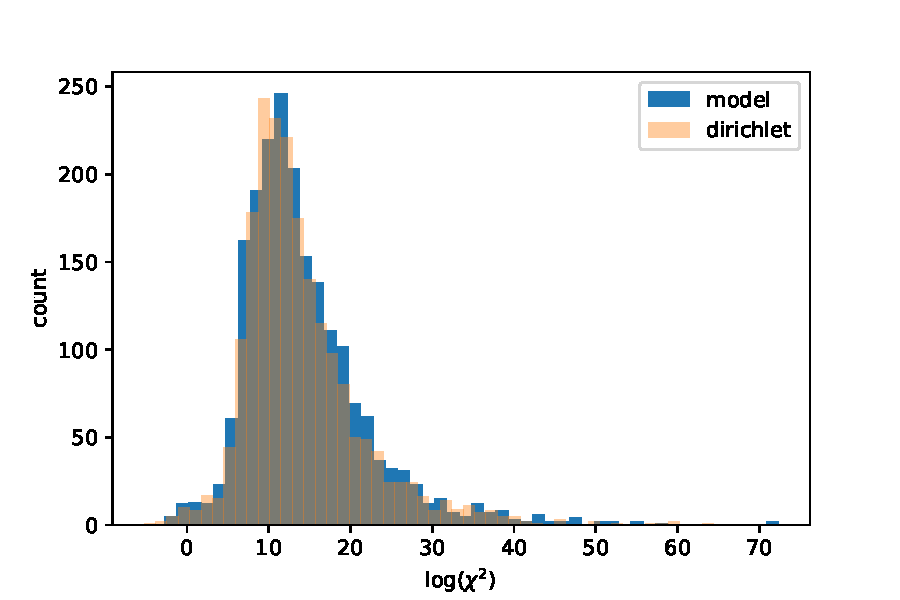
\includegraphics[width=\linewidth]{../figures/chi_square_stats/chi_hist_homogenous_0_01.pdf}
    \end{subfigure}
    \begin{subfigure}[a]{0.3\textwidth}
    \subcaption{Error scale is 0.1}
    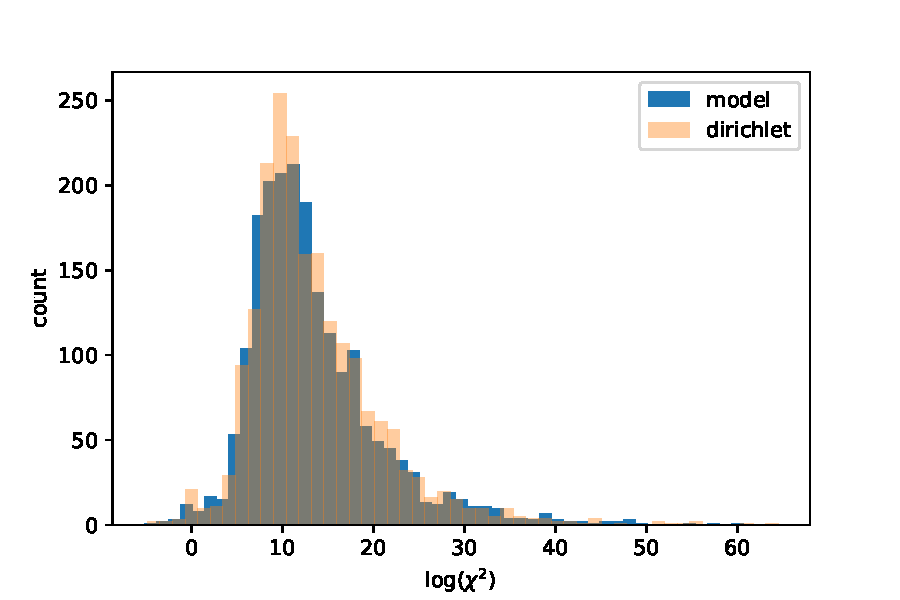
\includegraphics[width=\linewidth]{../figures/chi_square_stats/chi_hist_homogenous_0_1.pdf} 
    \end{subfigure}
    \begin{subfigure}[a]{0.3\textwidth}
     \subcaption{Error scale is 1(=J)}
    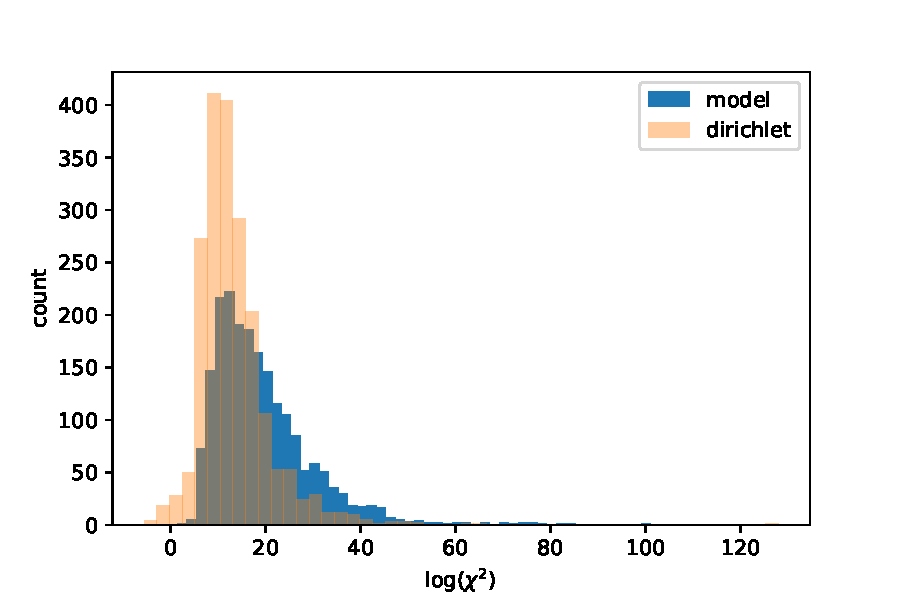
\includegraphics[width=\linewidth]{../figures/chi_square_stats/chi_hist_homogenous_J.pdf}
  \end{subfigure}
  \caption{Demonstrates the similarities between the $\chi ^2$ metric of 	           the DM approximation and the full model, showing the approximation is good until a very high error rate. Population size $N=2000$. 400 simulations per figure}	
  \label{fig:chiSquaredHist}
  \end{center}
\end{figure}


\subsection{Numeric comparisons}
We're interesting in studying the difference between the real binary model as we defined in \cref{eq:binary-model}, and the Dirichlet-Multinomial approximation. Specifically, we're interesting in the fixation probability of the favored trait ($\hat{A}$) and its time to fixation.

\begin{figure}
    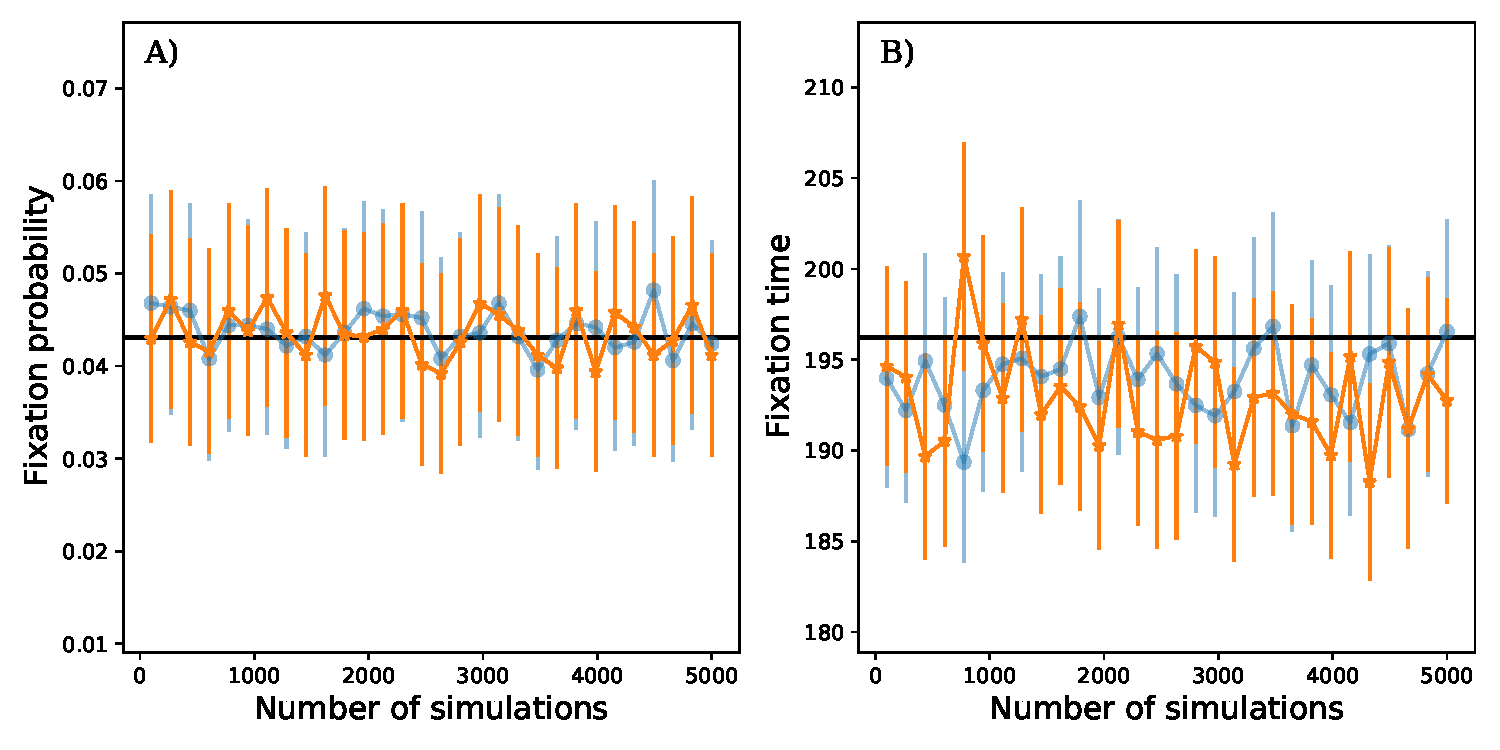
\includegraphics[width=\linewidth]{../figures/binary/num_sims.pdf}
  \caption{The number of simulations needed to get a good approximation. At $1,000$ the approximation is good enough. Error bars represent 95\% confidence interval. Population size $N=1000$, $\alpha=0.5$, $J=1$, $\hat{A}=1$,$A=0.7$, $\beta(A)=0.956$.}	
  \label{fig:num_sims}
\end{figure}


The first step was to find the number of simulations needed to sufficiently approximate the real model with the DM approximation. From \cref{fig:num_sims} we see that $1000$ simulations or higher is enough.

The next step was to see how the observed metrics (fixation probability and time) varies when relaxing our assumptions we used to prove the DM approximation.
First we relaxed our assumption of no mutation. To include mutation in the binary model, it needs to be redefined, since in the original model it was based on the fact the traits are drawn from a continuous scale. In the binary model mutation will be manifested as an error when evaluating the bias itself. This is easily done by using a heterogeneous $J$ parameter, which controls the strength of the success bias in \cref{eq:success_bias}.


\begin{figure}
    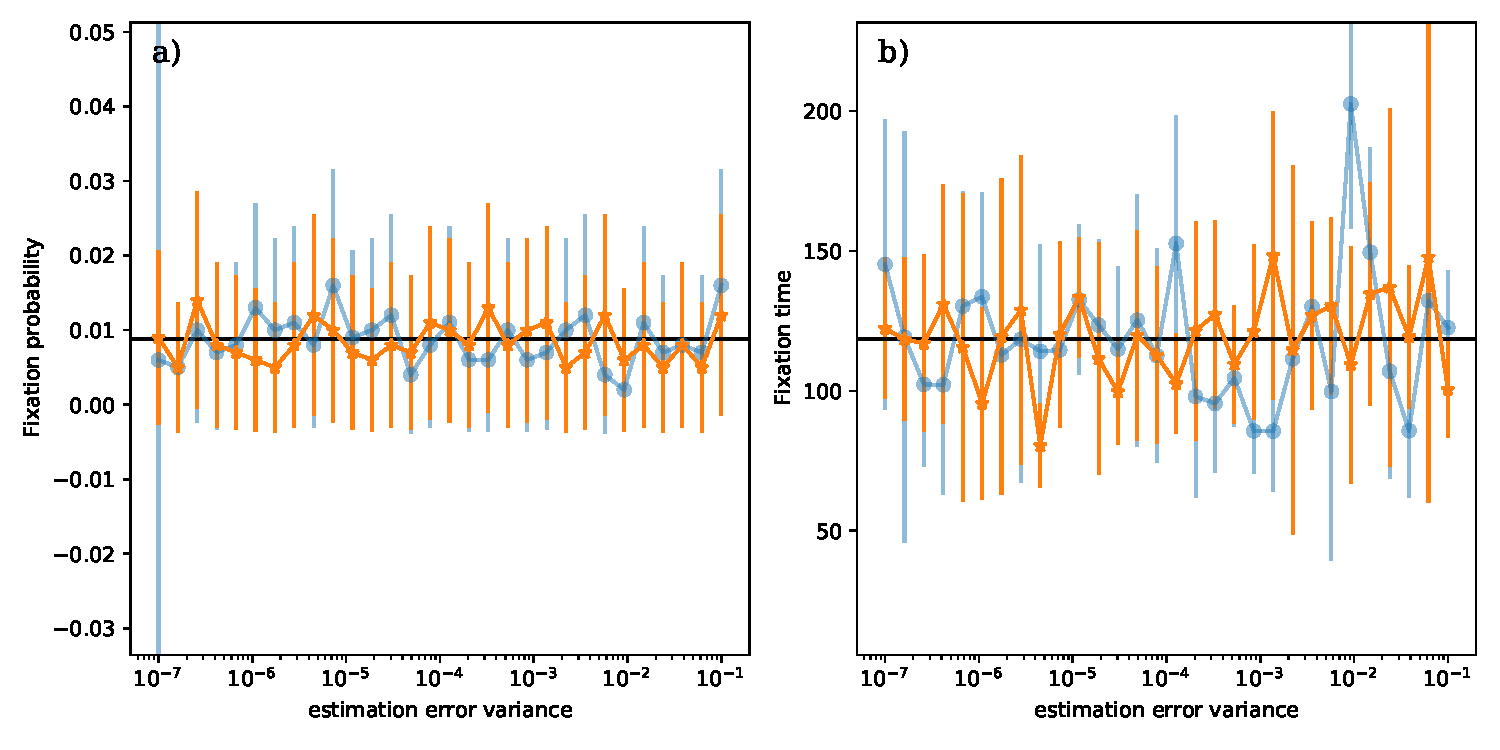
\includegraphics[width=\linewidth]{../figures/binary/full_vs_dm_mutation.pdf}
  \caption{Comparison of the DM approximation and the full model when mutation is included. Even high mutation rate doesn't worsen the approximation, and the data points are close to the mathematical estimation (Kimura's). Error bars are 95\% confidence intervals, and are condensed (+- 0.01 probability and +-40 generations)
  $5000$ simulations per data point, $N=1000$, $\alpha=0.1$,$\hat{A}=1$,$A=0.7$, $J\sim N(1,x^2)$ where $x$ is the mutation scale in the x-axis.
  }	
  \label{fig:hetro_mutation}
\end{figure}


In \cref{fig:hetro_mutation} we see the comparison when heterogeneous mutation is applied to both models. When mutation is applied, we sample $J_i$ for each copier $i$ from a normal distribution with varying scale (variance).
We can see that even when the standard deviation is $0.1$, the metrics of both models are both similar, and close to the Kimura approximation (more details in the next section). 

\begin{figure}
    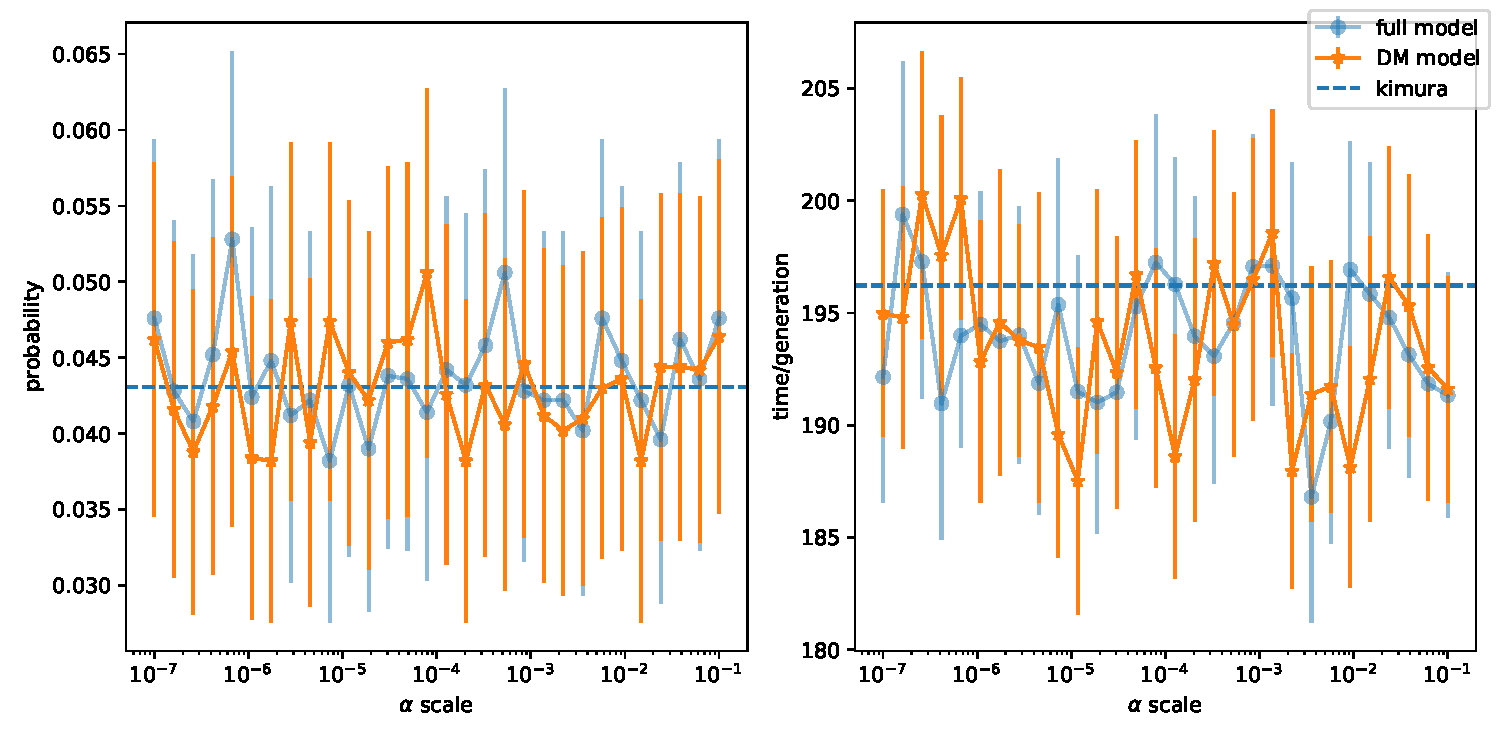
\includegraphics[width=\linewidth]{../figures/binary/full_vs_dm_changing_alpha.pdf}
  \caption{Comparison of the DM approximation and the full model when success weight is heterogeneous. High success weight variance distances the approximation and the full model of generations to fixation from the Kimura's approximation, but not by much (confidence intervals still cover it). Error bars are 95\% confidence intervals, and are less condensed (+- 0.03 probability and +-40 generations)
  $5000$ simulations per data point, $N=1000$, $\alpha\sim N(0.5,x^2)$,$\hat{A}=1$,$A=0.7$, $J=1$, $\beta(A)=0.956$.}	
  \label{fig:hetro_alpha}
\end{figure}

In \cref{fig:hetro_alpha} we relaxed our assumption of a homogeneous $\alpha$, and used a heterogeneous $\alpha$ instead. Similar to the mutation comparison, we drew $\alpha_j$ for each role-model $j$ from a normal distribution with varying scale. We again see that the metrics of both models are similar in the entire spectrum of our x-axis, and the Kimura approximation is within both confidence intervals.

\subsection{Fixation probability and time - binary model}
\paragraph{Kimura's approximation:}
After establishing a case in the favor of our DM approximation, we wanted to use it to examine the behavior of the population. Specifically, we wanted to analyze the influence of the indicator weight ($\alpha$) on the fixation probability and time to fixation of the favored phenotype in a binary model.
For simplicity, we don't include mutation rate in the binary model approximations.
Following \citet{durret}, we used our DM approximation of the model to find the effective population size. From \cref{eq:binary-model} we can derive that the process of inheritance in our binary model is DM distributed with a parameters vector of size two: $\vec{V}=(\alpha'X,(N-X)\alpha'\beta(A))$.

\paragraph{Proposition:} $1-\beta(A)$ is equivalent to the selection coefficient $s$ in a classic Wright-Fisher model in the diffusion equations meant to approximate the fixation probability and time of the advantageous trait.

\paragraph{Proof:} Let $x$ be the frequency of type $\hat{A}$ in the population with $N$ individuals. Let $X$ be the number of individuals of type $\hat{A}$ so $x=X/N$. $X'$ is the number of individuals with $\hat{A}$ in the next generation and $x'$ their frequency.
By definition $\beta(\hat{A})=1$, and for simplicity we'll denote $\beta(A)=\beta$ ($\beta<1$).

The expected number of individuals of a DM distribution is:
\begin{equation}
E[X'] = N  \frac{\alpha_1}{\alpha_1+\alpha_2},
\end{equation}
where $\alpha_1 = \alpha' X$ and $\alpha_2 = \alpha'(N-X)\beta$, from  \cref{eq:binary-model}.
We want to use frequencies instead of quantities to follow Durret's process so:
\begin{equation}
E[x'] = E[\frac{X'}{N}] = \frac{1}{N}E[X']
\end{equation}
Putting it together we get:
\begin{equation}
\begin{split}
E[x'] &= \frac{1}{N}N\frac{\alpha' xN}{\alpha' xN + \alpha' N (1-x)\beta}\\
	 &= \frac{x}{x + (1-x)\beta}
\end{split}
\end{equation}

which is identical to the equation in the top of page 253, chap 7.2 in \citet{durret}. We therefore use the same approximation and say that:
\begin{equation}
\begin{split}
E[x'] =& \frac{x}{x + (1-x)\beta} = \frac{x}{x + (1-x)(1-s)} =\\
 &= x + x(1-x)s + o(s)\\
  &= x + x(1-x)(1-\beta) + o(1-\beta)
\end{split}
\end{equation}

By definition, $x$ is constant, so $E[x] = x$. We continue to calculate $E[x'-x]$:
\begin{equation}\label{eq:expec_freq}
E[x'-x] = E[x'] - E[x] = x(1-x)(1-\beta) + o(1-\beta)
\end{equation}
where when substituting $1-\beta$ with $s$, we get the same result as \citet{durret} which is the desired result.

\paragraph{Proposition:} $Ne=\alpha N + (1-\alpha)$, where $Ne$ is the effective population size of our binary model.

\paragraph{Proof:} The variance of a DM distribution is:
\begin{equation}
V(X') = N\frac{\alpha_1}{\alpha_1+\alpha_2}(1-\frac{\alpha_1}{\alpha_1+\alpha_2})
(\frac{N + \alpha_1+\alpha_2}{1+\alpha_1+\alpha_2})
\end{equation}
And again, we want to use frequencies so:
\begin{equation}
V(\frac{X'}{N}) = \frac{1}{N^2}V(x')
\end{equation}

Putting it together with our model's notations:
\begin{equation}
V(x') = \frac{1}{N^2}N\frac{x}{x+(1-x)\beta}(1-\frac{x}{x+(1-x)\beta})
(\frac{N + \alpha' xN + \alpha' N(1-x)\beta}{1 + \alpha' xN + \alpha' N(1-x)\beta}) 
\end{equation}

Like Durret, we'll use the zero order of the approximation when $\beta\approx1$,so:
\begin{equation}
\frac{x}{x + (1-x)\beta} \approx x
\end{equation}
and we also use $\beta\approx1$ for the entire variance expression and get:
\begin{equation}
\begin{split}
V(x') & \approx  \frac{1}{N} x(1-x)
(\frac{N + \alpha' xN + \alpha' N - \alpha' xN}{1 + \alpha' xN + \alpha' N - \alpha' xN})\\
&=  x(1-x)(\frac{1 + \alpha'}{1 + \alpha' N}) 
\end{split}
\end{equation}

Again following Durret we want to calculate:
\begin{equation}\label{eq:var_diff_durret}
V(x'-x) = V(x') - V(x) \approx  x(1-x)(\frac{1 + \alpha'}{1 + \alpha' N})
\end{equation}
because $x$ is a constant so $V(x) = 0$

In our model, $\alpha'$ is the odds ratio of a parameter we called "indicator weight", denoted in our model as $\alpha$, so:
\begin{equation}\label{eq:success_ratio}
\alpha' = \frac{\alpha}{1-\alpha}
\end{equation}

Combining \cref{eq:var_diff_durret} and \cref{eq:success_ratio} we get:
\begin{equation}\label{eq:const_var}
\begin{split}
V(x'-x) & \approx x(1-x)(\frac{1 + \frac{\alpha}{1-\alpha}}{1 + \frac{\alpha}{1-\alpha} N})\\
 &= x(1-x)(\frac{\frac{1-\alpha+\alpha}{1-\alpha}}{\frac{1-\alpha+\alpha N}{1-\alpha}})\\
 &= x(1-x)(\frac{1}{1- \alpha(1-N)})\\
  &= x(1-x)(\frac{1}{\alpha N + (1-\alpha)})\\
  &= x(1-x)\frac{1}{N_e}
\end{split}
\end{equation}

Using our substitute for a selection coefficient, $1-\beta$, and the effective population size $N_e$, we can estimate the fixation probability and time of our binary model.

The fixation probability derived from Kimura is therefore:
\begin{equation}\label{eq:kimura_p}
P_{fix} = \frac{1-e^{-2(1-\beta)N_e x}}{1-e^{-2(1-\beta)N_e}}
\end{equation}

where $x$ is the initial frequency of the advantageous phenotype $\hat{A}$.

The time to fixation can be estimated by:
\begin{equation}\label{eq:kimura_t}
T_{fix}=\frac{1-P_{fix}}{1-\beta}\int_0^x\frac{e^{2(1-\beta) \xi}-1}{\xi(1-\xi)}d\xi+ \frac{P_{fix}}{1-\beta}\int_x^1\frac{1-e^{-2(1-\beta)(1-\xi)}}{\xi(1-\xi)}d\xi
\end{equation}
where the integrals cannot be solved in closed form, so we can only estimate them numerically.

To validate our math we ran multiple simulations comparing our binary model with the classic Wright-Fisher model, using different $\alpha$ and $\beta$ each time, and using the corresponding values of $s$ and $N_e$ for the WF simulations.
In \cref{fig:var_alpha} we changed $\alpha$ (and $N_e$ accordingly) and used a constant $\beta$.
In \cref{fig:var_beta} we changed $\beta$ and used a constant $\alpha$.
In both cases we can see that the two models behave similarly, and both are approximated well by the Kimura's equations: \cref{eq:kimura_p} and \cref{eq:kimura_t}.


\begin{figure}[t]
  \begin{center}
  \begin{subfigure}[a]{0.49\linewidth}
    \caption{}
    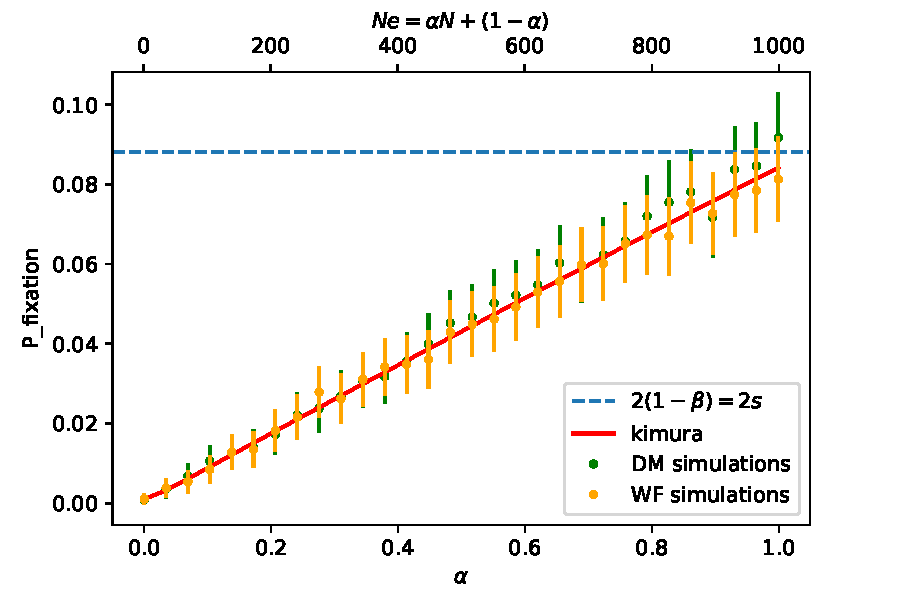
\includegraphics[width=\linewidth]{../figures/binary/fix_prob_var_alpha.pdf}
   \end{subfigure}
   \begin{subfigure}[a]{0.49\linewidth}
     \caption{}
    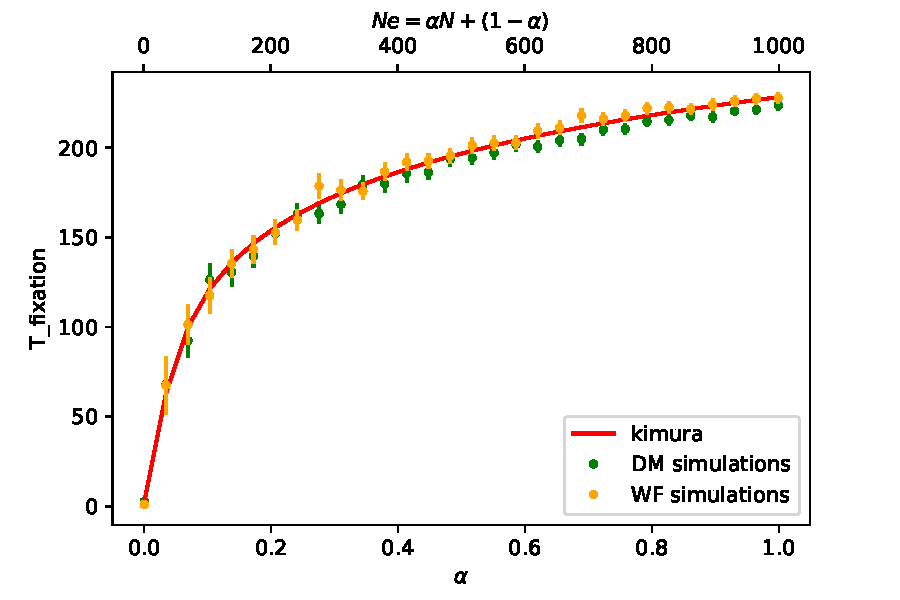
\includegraphics[width=\linewidth]{../figures/binary/fix_time_var_alpha.pdf}
   \end{subfigure}
  \end{center}
  \caption{Comparison of the DM approximation and the WF model for different values of the effective population size. The approximation seems very good, and is also condensed around the mathematical equation expectancy. Error bars are 95\% confidence intervals.
  Effective population calculated by $N_e=\alpha N + (1-\alpha)$.
  $5,000$ simulations per data point, $N=1,000$, $\hat{A}=1$, $A=0.7$,$J=1$,$1-\beta=s=0.044$.}
  \label{fig:var_alpha}
\end{figure}

\begin{figure}[t]
  \begin{center}
  \begin{subfigure}[a]{0.49\linewidth}
  \caption{}
    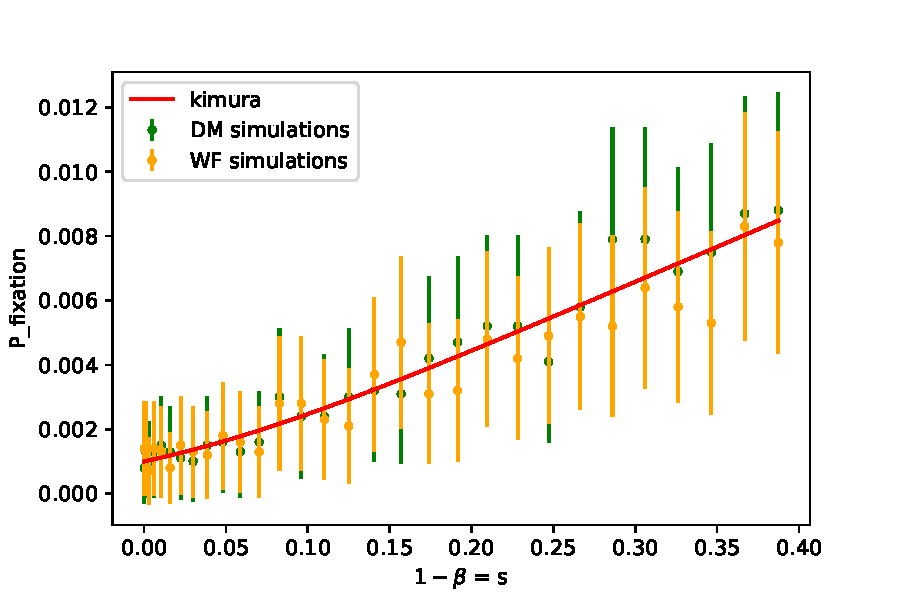
\includegraphics[width=\linewidth]{../figures/binary/fix_prob_var_beta.pdf}
   \end{subfigure}
   \begin{subfigure}[a]{0.49\linewidth}
    \caption{}
    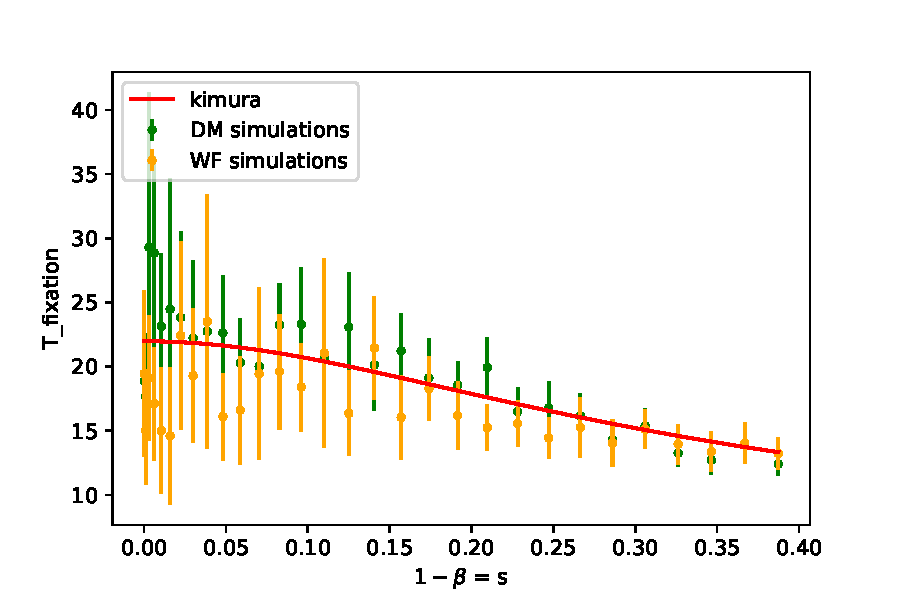
\includegraphics[width=\linewidth]{../figures/binary/fix_time_var_beta.pdf}
   \end{subfigure}
  \end{center}
  \caption{Comparison of the DM approximation and the WF model for different values of the selection coefficient, manifested as success bias in our model. The approximation seems good, and is also condensed around the mathematical equation expectancy. Error bars are 95\% confidence intervals.
  Effective population calculated by $N_e=\alpha N + (1-\alpha)$.
  $5,000$ simulations per data point, $N=1,000$, $\hat{A}=1$, $A=0.7$,$J=1$,$\alpha=0.01$.}
  \label{fig:var_beta}
\end{figure}

\subsection{Changing environment}
After finding good estimations for our model in a constant environment, when the favorable trait is always $\hat{A}$, we want to find an estimation for our model in a changing environment.

For that we will find an expression for the expected and variance of the change in frequency between $t$ generations.
Let $s_t=N(1-\beta_t)$, and $S_n=\sum\limits_{i=1}^n s_i$, where $\beta_t$ is $\beta(A)$ at time/generation $t$.


\paragraph{Proposition:} $E[\frac{X_t}{N}-x]\simeq \frac{1}{N}S_tx(1-x)$ , $V(\frac{X_t}{N})\simeq\frac{1}{N_e}tx(1-x)$, where $x$ is the initial frequency of the favorable/invading trait and $X_t$ is the number of individuals with the trait at time $t$.

The proof is based on the proof of \citet{changeEnv}, proving a similar scenario.
\paragraph{Proof by induction:}
From \cref{eq:expec_freq} we know that
\begin{equation}\label{eq:ch_1}
\begin{split}
E\left[\frac{X_{t+1}}{N}-\frac{X_t}{N}\bigg|X_t\right] &= \frac{X_t}{N}\left(1-\frac{X_t}{N}\right)(1-\beta_{t+1}) \\
&= \frac{1}{N}\frac{X_t}{N}\left(1-\frac{X_t}{N}\right)s_{t+1}
\end{split}
\end{equation}
Also note that using the definition of $V(y)=E[y^2]-(E[y])^2$
\begin{equation}
\begin{split}
E\left[\frac{X_t}{N}\left(1-\frac{X_t}{N}\right)\right] &= E\left[\frac{X_t}{N}-\left(\frac{X_t}{N}\right)^2\right] \\
&= E\left[\frac{X_t}{N}\right]-E\left[\left(\frac{X_t}{N}\right)^2\right] \\
&= E\left[\frac{X_t}{N}\right] - V\left(\frac{X_t}{N}\right) - \left(E\left[\frac{X_t}{N}\right]\right)^2
\end{split}
\end{equation}

we can now use the induction assumption of $V(\frac{X_t}{N})$ and get
\begin{equation}
\begin{split}
E\left[\frac{X_t}{N}\left(1-\frac{X_t}{N}\right)\right] &\simeq
E\left[\frac{X_t}{N}\right]\left(1-E\left[\frac{X_t}{N}\right]\right)-\frac{1}{N_e}tx(1-x)
\end{split}
\end{equation}
From \cref{eq:ch_1} we know that
\begin{equation}
\begin{split}
E\left[\frac{X_{t+1}}{N}-\frac{X_t}{N}\right] &= \frac{1}{N}s_{t+1}E\left[\frac{X_t}{N}\left(1-\frac{X_t}{N}\right)\right] \\
&\simeq \frac{1}{N}s_{t+1}\left(E\left[\frac{X_t}{N}\right]\left(1-E\left[\frac{X_t}{N}\right]\right) - \frac{1}{N_e}tx(1-x)\right) \\
&\simeq \frac{1}{N}s_{t+1}\cdot E\left[\frac{X_t}{N}\right]\left(1-E\left[\frac{X_t}{N}\right]\right) - \frac{1}{N_e N}s_{t+1}tx(1-x)
\end{split}
\end{equation}
Now we'll omit $O(\frac{1}{Ne\cdot N})$ and get
\begin{equation}\label{eq:ch_2}
E\left[\frac{X_{t+1}}{N}-\frac{X_t}{N}\right] \simeq \frac{1}{N}s_{t+1}\cdot E\left[\frac{X_t}{N}\right]\left(1-E\left[\frac{X_t}{N}\right]\right)
\end{equation}

We'll now look at the induction assumption to see that
\begin{equation}
E\left[\frac{X_t}{N}-x\right]=E\left[\frac{X_t}{N}\right]-E[x]=E\left[\frac{X_t}{N}\right]-x ,
\end{equation}
so using the assumption we get
\begin{equation}
\begin{split}
E\left[\frac{X_t}{N}\right] &\simeq \frac{1}{N} S_t x(1-x)+x \\
1 - E\left[\frac{X_t}{N}\right] &\simeq 1- \frac{1}{N} S_t x(1-x)+x
\end{split}
\end{equation}
we'll use both expressions in \cref{eq:ch_2} and get
\begin{equation}\label{eq:ch_3}
\begin{split}
E\left[\frac{X_{t+1}}{N}-\frac{X_t}{N}\right] &\simeq \frac{1}{N}s_{t+1} \left(\frac{1}{N} S_t x(1-x)+x \right)\left(1- \frac{1}{N} S_t x(1-x)+x \right) \\
&\simeq  \frac{1}{N}s_{t+1}\cdot x(1-x)
\end{split}
\end{equation}
after again omitting $O(\frac{1}{N^2})$ parts of the equation.
To conclude our proof, we see that
\begin{equation}
E\left[\frac{X_{t+1}}{N}-x\right] = E\left[\frac{X_{t+1}}{N}-\frac{X_t}{N}\right] + E\left[\frac{X_t}{N}-x\right]
\end{equation}
so again using the induction assumption, together with \cref{eq:ch_3} we get
\begin{equation}
\begin{split}
E\left[\frac{X_{t+1}}{N}-x\right] &\simeq \frac{1}{N}s_{t+1}\cdot x(1-x) + \frac{1}{N}S_t\cdot x(1-x) \\
& \simeq \frac{1}{N}x(1-x)(S_t + s_{t+1}) \\
& \simeq \frac{1}{N} S_{t+1} x(1-x)
\end{split}
\end{equation}
which proves the first part of our preposition.

For the second part, we'll use a property of variance:
\begin{equation}\label{eq:ch_var}
V\left(\frac{X_{t+1}}{N}\right) = E\left[V\left(\frac{X_{t+1}}{N} \bigg|X_t \right)\right] + V\left(E\left[\frac{X_{t+1}}{N} \bigg|X_t \right]\right)
\end{equation}

using \cref{eq:ch_1} we see that:
\begin{equation}\label{eq:ch_var1}
\begin{split}
E\left[\frac{X_{t+1}}{N} \bigg|X_t \right] - E\left[\frac{X_{t}}{N} \bigg|X_t \right] &= \frac{1}{N}s_{t+1}\frac{X_t}{N}\left(1-\frac{X_t}{N} \right) \\
E\left[\frac{X_{t+1}}{N} \bigg|X_t \right] = \frac{X_t}{N} &+ \frac{1}{N}s_{t+1}\frac{X_t}{N}\left(1-\frac{X_t}{N} \right)
\end{split}
\end{equation}

Using \cref{eq:const_var} we get:
\begin{equation}
V\left(\frac{X_{t+1}}{N} \bigg|X_t \right) = \frac{1}{N_e}\frac{X_t}{N}\left(1-\frac{X_t}{N} \right)
\end{equation}

and using the equation $y'(1-y') \simeq y(1-y)$ on the first part of \cref{eq:ch_var} we get:
\begin{equation}\label{eq:ch_var2}
E\left[V\left(\frac{X_{t+1}}{N} \bigg|X_t \right)\right] = \frac{1}{N_e}E\left[\frac{X_t}{N}\left(1- \frac{X_t}{N}\right) \right] \simeq \frac{1}{N_e} x(1-x)
\end{equation}

and moving on to simplify the second part of \cref{eq:ch_var} using \cref{eq:ch_var1}:
\begin{equation}
V\left(E\left[\frac{X_{t+1}}{N} \bigg|X_t \right]\right) = V\left(\frac{X_t}{N} + \frac{1}{N}s_{t+1}\frac{X_t}{N}\left(1-\frac{X_t}{N} \right) \right)
\end{equation}

and now, because $\frac{X_t}{N}$ is a frequency, i.e $0\leq\frac{X_t}{N}\leq1$, we know that $V\left(\frac{X_t}{N}\left(1-\frac{X_t}{N} \right) \right)\leq\frac{1}{4}$. We therefore see that:
\begin{equation}
V\left(\frac{1}{N}s_{t+1}\frac{X_t}{N}\left(1-\frac{X_t}{N} \right) \right)\leq \frac{1}{4N^2}s^2_{t+1}
\end{equation}
and so it can be ignored.
Combining our equations we get:
\begin{equation}
V\left(E\left[\frac{X_{t+1}}{N} \bigg|X_t \right]\right) = V\left(\frac{X_t}{N}\right) + O\left(\frac{1}{N^2}\right)\simeq V\left(\frac{X_t}{N}\right)
\end{equation}

Using the induction assumption and \cref{eq:ch_var2}:
\begin{equation}
V\left(\frac{X_{t+1}}{N}\right) \simeq \frac{1}{N_e}x(1-x) + \frac{1}{N_e}tx(1-x) \simeq \frac{1}{N_e}x(1-x)(t+1)
\end{equation}
proving the second part of our preposition.

Following our proof, we can say that after many cycles, we can use a modified version of our fixation probability:
\begin{equation}
P_{fix} = \frac{1-e^{-2 \frac{S_n}{n} N_e x}}{1-e^{-2 \frac{S_n}{n} N_e}}
\end{equation}
where $\frac{S_n}{n} = \frac{k-l}{k+l}(1-beta)$, $n=k+l$. Put into words, we use the average selection coefficient of a cycle ($k+l$) as the selection coefficient in our original equation.
In our proof we showed that the expected change in frequency and variance is only manifested in the selection coefficient $S_n$, and that we can use those modified equation as a base for Kimura's equation.

We wanted again to validate our results, using simulations.
This time, the number of parameters increased: in addition to $\alpha,\beta$, there are also $k,l$ as model parameters.

We again tried different variations of the parameters, changing only one of them at a time.
In \cref{fig:ch_env_alpha_beta} we can see that $\alpha$ on it's own doesn't cause any deviation for the the estimation. $\beta$ however affects the results greatly.

\begin{figure}[t]
  \begin{center}
  \begin{subfigure}[a]{0.49\linewidth}
  \caption{success bias/selection coefficient is: $1-\beta=s=0.005$}
    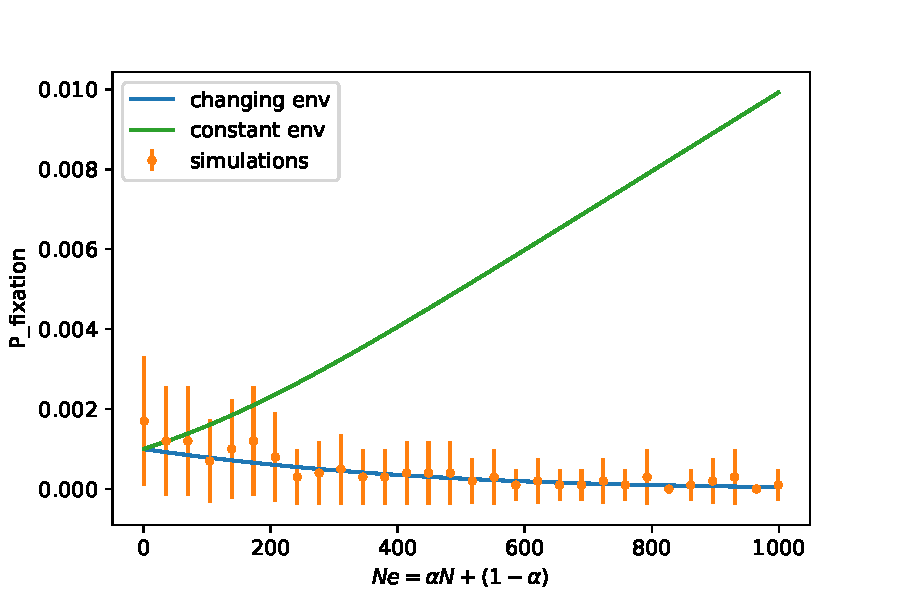
\includegraphics[width=\linewidth]{../figures/changed_env/ch_env_var_alpha.pdf}
   \end{subfigure}
   \begin{subfigure}[a]{0.49\linewidth}
   \caption{success weight is: $\alpha=0.1$}
    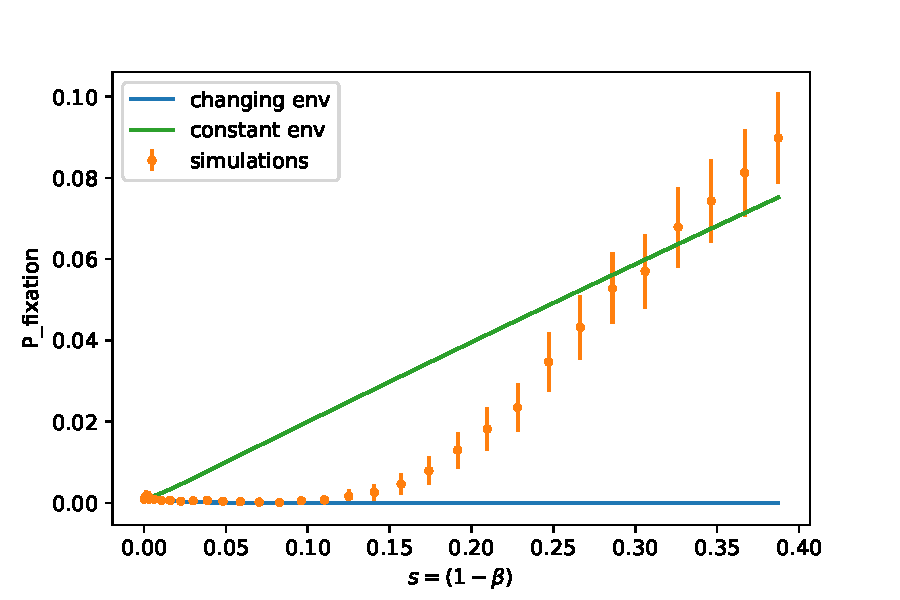
\includegraphics[width=\linewidth]{../figures/changed_env/ch_env_var_beta.pdf}
   \end{subfigure}
  \end{center}
  \caption{Model simulations compared with both the constant environment and the changing environment equations with different effective populations sizes and selection coefficients. Changing the effective population size doesn't affect the approximation, and it is condensed the mathematical expected values across all values. High values of success bias ($s>0.1$) will distance the simulations from the changing environment expected values. Very high values ($s>0.35$) will even deviate from the constant environment expected values. This is expected because Kimura's approximation are only viable for low selection coefficient values.
  $10,000$ simulations per data point, $N=1,000$, $\hat{A}=1$, $A=0.9$, $J=1$.}
  \label{fig:ch_env_alpha_beta}
\end{figure}

We plotted along the modified estimation the original Kimura's estimation, as a limiter. We suspect that when $\beta$ is too large, there won't be many cycles in the simulations. This might happen if either the population reaches a high frequency of the ideal trait after only a few cycles, or it get extinct very quickly, because the advantage it had in the $k$ generations wasn't sufficient, and the same $s$ becomes a greater disadvantage when the environment changes, resulting in a fast extinction.

In the larger values of $beta$ we even see a deviation from the original estimation environment, but it's to be expected, because Kimura's equations are only viable for small $s$ values.

We then also tried changing the composition of the cycle, by keeping a constant $n=40$, but changing $k,l$ accordingly.

\begin{figure}[t]
  \begin{center}
  \begin{subfigure}[a]{0.49\linewidth}
  \caption{}
    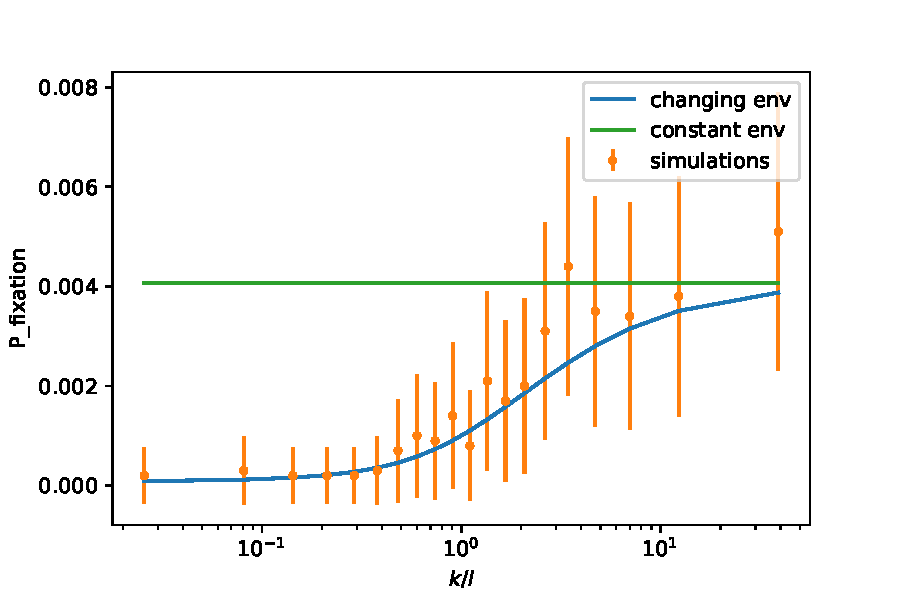
\includegraphics[width=\linewidth]{../figures/changed_env/ch_env_var_k_div_l.pdf}
   \end{subfigure}
   \begin{subfigure}[a]{0.49\linewidth}
   \caption{}
    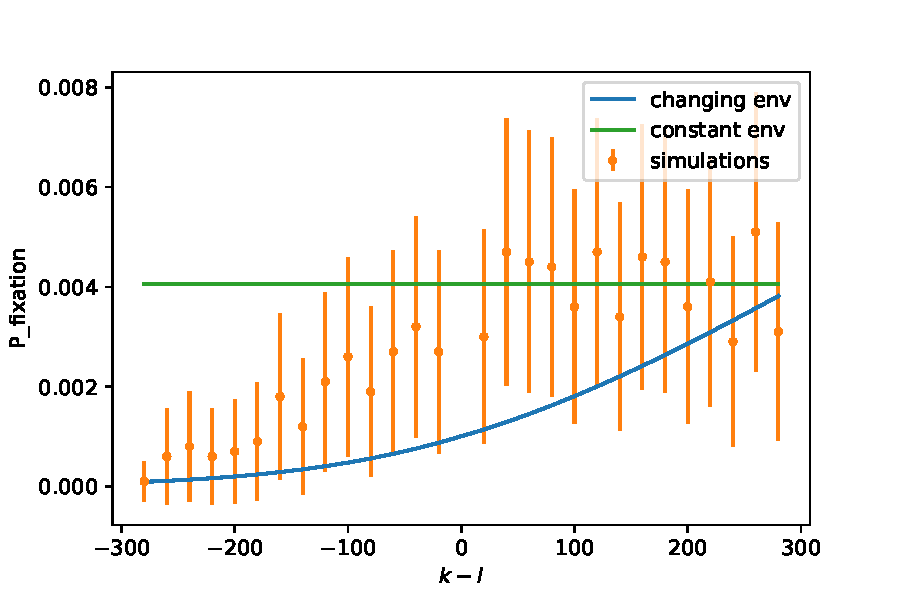
\includegraphics[width=\linewidth]{../figures/changed_env/ch_env_var_k_min_l.pdf}
   \end{subfigure}
  \end{center}
  \caption{Model simulations compared with both the constant environment and the changing environment equations for different compositions of the environment cycle. When $k<l$ the approximation is good. When $k>l$, the approximation and the simulations are both very close to the constant environment approximation. 
  $10,000$ simulations per data point, $N=1,000$, $\hat{A}=1$, $A=0.8$, $J=1$, $1-\beta=s=0.02$, $\alpha=0.1$.}
  \label{fig:ch_env_k_l}
\end{figure}

In \cref{fig:ch_env_k_l} we see that the larger $k$ relative to $l$, the closer the modified equation is to the original estimation of the constant environment. 
When using higher values of $n$, the simulation results doesn't fit the equation result as with lower values. This is due to the fact that our proof, and therefore our equation is more accurate when more cycles occur. When $n$ is high, there will be less cycles, and the simulations will get closer to the constant environment equation.

\section{Discussion}
Cultural transmission is the phenomenon of which cultural elements, in the form of attitudes, values, beliefs, and behavioral patterns, are transmitted between individuals, typically via copying.
Some cultural traits can be more likely to be copied by others, regardless of their frequency in the population.  
Such transmission biases are common in cultural transmission processes. 
Many models are based on the assumption that success can be correctly identified, and easily copied.
Here we assume that success isn't correctly identified, therefore individuals may use other indicators to try and estimate the success of potential role-models.
We believe, as \citet{complexityPaper} suggest, that \textit{prestige biases} are more common in nature than success biases, since estimating success is harder.
We believe prestige is composed of two main components: a trait that indicates success (but doesn't guarantee it), and the influence the individual already has on others, i.e number of individuals already chose him as a role-model.
We suggest a model for \textit{prestige bias}, inspired by the model \citet{evolutionBook} have suggested, and added the \textit{influence bias} to it.
We approximated our models using various distributions, and compared them to the original model using simulations.
We showed that a \textit{Rich getting richer} type of model can be approximated well by the general binomial distribution and the dirichlet multinomial distribution.
We experimented with constant and changing environment in our model, and created a variation of a binary model for easier mathematical and computational analysis.
We believe that in this era of social media it is easy to estimate one's influence over others.
It is therefore crucial to model the cultural biases more realistically than success bias based model, and we believe including influence is crucial for that purpose.\\
With a more realistic model of a common cultural transmission bias, we may be able to better understand decision-making processes in humans, including life-changing choices such as occupation or a life partner. 
Our model can be expanded in multiple ways: observing the effects of different bias functions, including errors in estimating the influence, combining factors of cost when copying from an influential role model (not all could afford to copy from the most popular role-model), and analyzing the differences when including several optimal values for the indicator trait (multiple preference traits in the population).

\clearpage
\section{Appendix A - Time table}

\paragraph{Today - Oct 2021:}
Find approximation replacing Durrett's equations for the time to fixation.

\paragraph{Nov - Mar 2021:}
Combining the findings to a paper and a thesis.



\clearpage
\bibliography{refs}
\bibliographystyle{apalike}
\end{document}
